% 2014 全国卷Ⅰ理科第 12 题：小正方形边长为 1 的三视图。
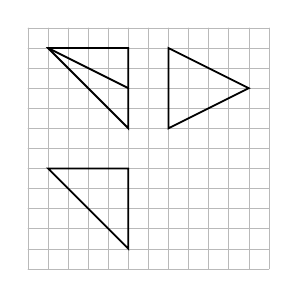
\begin{tikzpicture}[x=2.55mm,y=2.55mm,line cap=round]
  \draw[step=1,gray!55,line width=.18pt] (0,0) grid (12,12);
  % 左上投影：两条斜边从同一顶点出发。
  \draw[line width=.65pt] (1,11)--(5,11)--(5,7)--cycle;
  \draw[line width=.65pt] (1,11)--(5,9);
  % 右上投影：指向右侧的三角形投影。
  \draw[line width=.65pt] (7,11)--(11,9)--(7,7)--cycle;
  \draw[line width=.65pt] (7,11)--(7,7);
  % 左下投影：斜线三角形。
  \draw[line width=.65pt] (1,5)--(5,5)--(5,1)--cycle;
\end{tikzpicture}
